% Hlavicka pro protokoly z fyzikalniho praktika.
% Verze pro: LaTeX
% Verze hlavicky: 22. 2. 2007
% Autor: Ustav fyziky kondenzovanych latek
% Ke stazeni: www.physics.muni.cz/ufkl/Vyuka/
% Licence: volne k pouziti, nejlepe k vcasnemu odevzdani protokolu z Vaseho mereni.

\documentclass[a4paper,11pt]{article}

% Kodovani (cestiny) v dokumentu: utf-8
%\usepackage[cp1250]{inputenc}	% Omezena stredoevropska kodova stranka, pouze MSW.
\usepackage[utf8]{inputenc}	% Doporucujeme pouzivat UTF-8 (unicode).

%%% Nemente:
\usepackage[margin=2cm]{geometry}
\newtoks\jmenopraktika \newtoks\jmeno \newtoks\datum
\newtoks\obor \newtoks\skupina \newtoks\rocnik \newtoks\semestr
\newtoks\cisloulohy \newtoks\jmenoulohy
\newtoks\tlak \newtoks\teplota \newtoks\vlhkost
\usepackage{amsmath}
\usepackage{mathtools}
\usepackage{graphicx}
\usepackage{multirow}
\graphicspath{ {./images/} }
%%% Nemente - konec.


%%%%%%%%%%% Doplnte pozadovane polozky:

\jmenopraktika={Fyzikální praktikum 2}  % nahradte jmenem vaseho predmetu
\jmeno={Artem Gorodilov}            % nahradte jmenem mericiho
\datum={23. ~listopadu  2023}        % nahradte datem mereni ulohy
\obor={Astrofyzika}                     % nahradte zkratkou vami studovaneho oboru
\skupina={Čt 8:00}            % nahradte dobou vyuky vasi seminarni skupiny
\rocnik={II}                  % nahradte rocnikem, ve kterem studujete
\semestr={I}                 % nahradte semestrem, ve kterem studujete

\cisloulohy={10}               % nahradte cislem merene ulohy
\jmenoulohy={Polarizace světla} % nahradte jmenem merene ulohy

\tlak={982}                   % nahradte tlakem pri mereni (v hPa)
\teplota={21.7}               % nahradte teplotou pri mereni (ve stupnich Celsia)
\vlhkost={39}               % nahradte vlhkosti vzduchu pri mereni (v %)

%%%%%%%%%%% Konec pozadovanych polozek.


%%%%%%%%%%% Uzitecne balicky:
\usepackage[czech]{babel}
\usepackage{graphicx}
\usepackage{amsmath}
\usepackage{xspace}
\usepackage{url}
\usepackage{indentfirst}
\usepackage{listings}
\usepackage{subcaption}
\usepackage{caption}
\usepackage{tabularx}
\usepackage[labelformat=parens,labelsep=quad,skip=3pt]{caption}

%%%%%% Zamezeni parchantu:
\widowpenalty 10000 \clubpenalty 10000 \displaywidowpenalty 10000
%%%%%% Parametry pro moznost vsazeni vetsiho poctu obrazku na stranku
\setcounter{topnumber}{3}	  % max. pocet floatu nahore (specifikace t)
\setcounter{bottomnumber}{3}	  % max. pocet floatu dole (specifikace b)
\setcounter{totalnumber}{6}	  % max. pocet floatu na strance celkem
\renewcommand\topfraction{0.9}	  % max podil stranky pro floaty nahore
\renewcommand\bottomfraction{0.9} % max podil stranky pro floaty dole
\renewcommand\textfraction{0.1}	  % min podil stranky, ktery musi obsahovat text
\intextsep=8mm \textfloatsep=8mm  %\intextsep pro ulozeni [h] floatu a \textfloatsep pro [b] or [t]

% Tecky za cisly sekci:
\renewcommand{\thesection}{\arabic{section}.}
\renewcommand{\thesubsection}{\thesection\arabic{subsection}.}
% Jednopismenna mezera mezi cislem a nazvem kapitoly:
\makeatletter \def\@seccntformat#1{\csname the#1\endcsname\hspace{1ex}} \makeatother

\begin{document}

\thispagestyle{empty}

{
\begin{center}
\sf 
{\Large Ústav fyzikální elektroniky PřF MU} \\
\bigskip
{\huge \bfseries FYZIKÁLNÍ PRAKTIKUM} \\
\bigskip
{\Large \the\jmenopraktika}
\end{center}

\bigskip

\sf
\noindent
\setlength{\arrayrulewidth}{1pt}
\begin{tabular*}{\textwidth}{@{\extracolsep{\fill}} l l}
\large {\bfseries Zpracoval:}  \the\jmeno & \large  {\bfseries Naměřeno:} \the\datum\\[2mm]
\large  {\bfseries Obor:} \the\obor  \hspace{40mm}  {\bfseries Skupina:} \the\skupina %
%{\bfseries Ročník:} \the\rocnik \hspace{5mm} {\bfseries Semestr:} \the\semestr  
&\large {\bfseries Testováno:}\\
\\
\hline
\end{tabular*}
}

\bigskip

{
\sf
\noindent \begin{tabular}{p{3cm} p{0.6\textwidth}}
\Large  Úloha č. {\bfseries \the\cisloulohy:} \par
\smallskip
$T=\the\teplota$~$^\circ$C \par
$p=\the\tlak$~hPa \par
$\varphi=\the\vlhkost$~\%
&\Large \bfseries \the\jmenoulohy  \\[2mm]
\end{tabular}
}

\vskip1cm
    \begin{minipage}[t]{0.5\textwidth} 
        \section{Zadání}
            Změřte index lomu roztoků sacharózy o různých koncentracích. 
            \par Změřte specifickou stáčivost roztoků.
            \par Změřte polarizovatelnost skutečného polaroidu pomocí Mazulova zákona.
        \section{Teorie}
            \subsection{Optická aktivita látek}
                Opticky aktivní látky, jako jsou některé pevné materiály a kapaliny s asymetrickým uhlíkem, například vodný roztok sacharózy, vykazují schopnost ohýbat rovinu lineární polarizace světla. V závislosti na směru natočení vibrační roviny se klasifikují jako pravotočivé nebo levotočivé vzhledem ke směru šíření světla. Úhel natočení roviny kmitání po průchodu opticky aktivní látkou popisuje rovnice:
                \begin{equation}
                    \alpha = [\alpha]d
                \end{equation}
                kde $[\alpha]$ je specifická specifická stáčivost zkoumané látky a $d$ je je tlošťka látky.
                \par Teplota a vlnová délka světla určují hodnotu [$\alpha$]. Specifická stáčivost $[\alpha]$ je definována jako:
                \begin{equation}
                    [\alpha] = \frac{\alpha}{cd}
                \end{equation}
                kde $c$ je koncentrace roztoku.
                \par Závislost úhlu lomu $n$ na malé (do 20\%) koncentraci $c$ popisuje následující vzorec: 
                \begin{equation}
                    n(c) = n_{voda} + (0.00140 \pm 0.00003)c
                \end{equation}
    \end{minipage}
    \hspace{10pt}
    \begin{minipage}[t]{0.5\textwidth} 
                \vspace{-10pt}
                \par \centering
                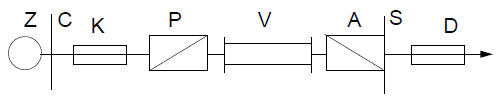
\includegraphics[scale=0.6]{polar}
                \captionsetup{justification=centering, font=footnotesize}
                \captionof{figure}{Polarimetr.}
                \label{fig:polar}
                \vspace{10pt}
                \raggedright
                \par kde $n_0$ je index lomu čistého rozpouštědla a $A$ je koeficient úměrnosti.
            \subsection{Malusův zákon}
                Prvky jsou znázorněny na schématu (1): $A$ - analyzátor a $P$ - polarizátor. $I_0$ - intenzita přirozeného světla dopadajícího na polarizátor. $I_0'$ je intenzita světla po průchodu polarizátorem. Dále $I$ je intenzita paprsku po průchodu analyzátorem $A$ a $\alpha$ je úhel mezi rovinami kmitání vektoru $\overrightarrow{E}$ před průchodem analyzátorem a po něm obrazek (2). 
                \par Nechť amplituda vektoru $\overrightarrow{E}$ před průchodem je $a_0$ a po průchodu je $a$. Pak platí následující:
                \begin{equation}
                    a = a_0 cos\alpha
                \end{equation}
                Intenzita prošlá analyzátorem je určena Malusovým zákonem:
                \begin{equation}
                    I = I_0 cos^2\alpha
                \end{equation}
                \par \centering
                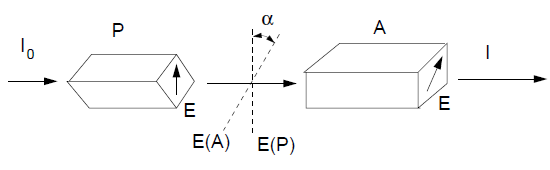
\includegraphics[scale=0.6]{mus}
                \captionsetup{justification=centering, font=footnotesize}
                \captionof{figure}{Shéma Malusova pokusu.}
                \label{fig:mus}
                \vspace{10pt}
                \raggedright
    \end{minipage}
\newpage
    \begin{minipage}[t]{0.5\textwidth} 
        \section{Měření}  
            \subsection{Optická aktivita látek}
                Refraktometrem byly změřeny indexy lomu $n$ pro diionizovanou vodu a pro 5\%, 10\% a 15\% concentrace $c$ roztoku sacharózy v této vodě. Výsledky jsou uvedeny v tabulce (1).  
                \vspace{10pt}
                \par \centering
                \begin{tabular}{|c|c|c|}
                    \hline
                    $c_0$ [\%] & $c$ [\%] & $n$ \\
                    \hline
                    0 & -0.1(3) & 1.332(1) \\
                    \hline
                    5 & 4.1(3) & 1.339(2) \\
                    \hline
                    10 & 7.8(4) & 1.346(1) \\
                    \hline
                    15 & 14.2(4) & 1.354(1) \\
                    \hline
                \end{tabular}
                \captionsetup{justification=centering, font=footnotesize}
                \captionof{table}{Indexy lomu $n$ pro různé naměřené koncentrace sacharózy $c$ odpovídající očekávaným koncentracím $c_0$.}
                \vspace{10pt}
                \raggedright
                \par Dále jsme vykreslili závislost indexu lomu na koncentraci roztoku a lineárně ji aproximovali, čímž jsme získali hodnotu $A$. Výsledky jsou uvedeny na obrázku (3). 
                \vspace{10pt}
                \par \centering
                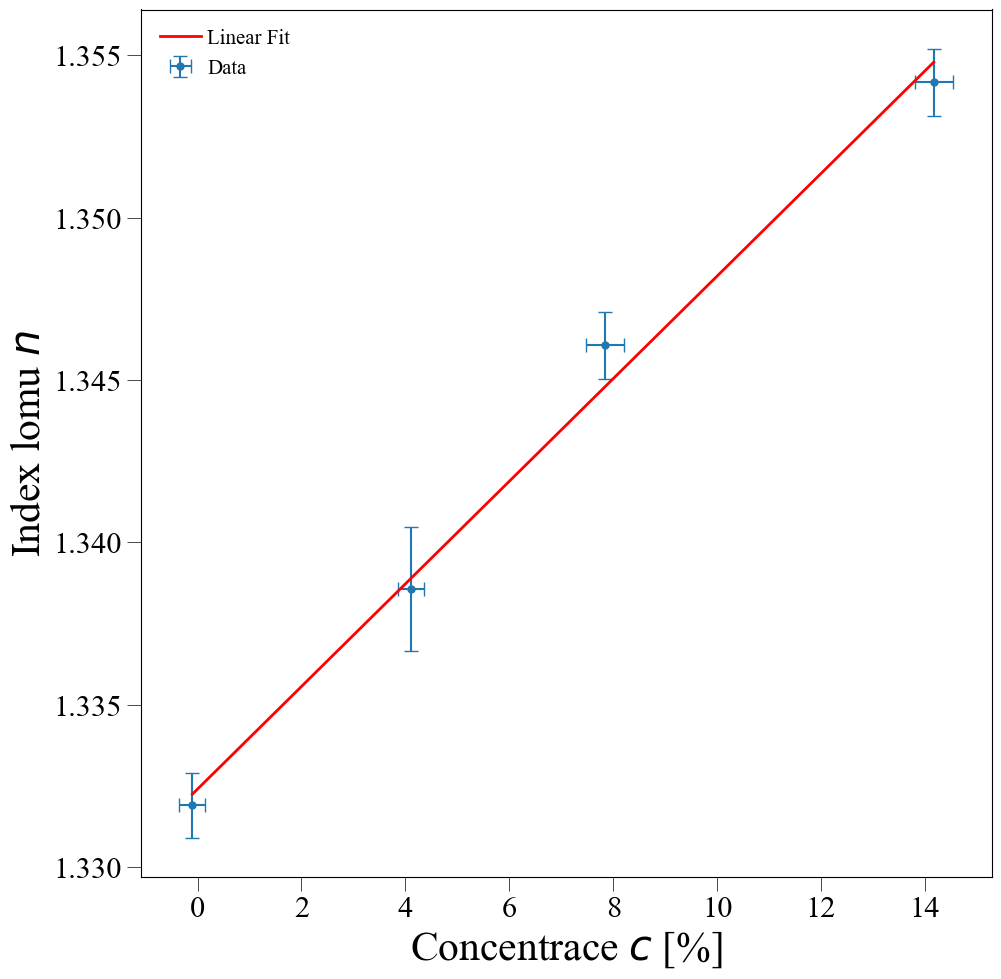
\includegraphics[scale=0.3]{lom}
                \captionsetup{justification=centering, font=footnotesize}
                \captionof{figure}{Závislost indexu lomu $n$ na koncentraci roztoku sacharózy $c$.}
                \label{fig:lom}
                \raggedright
                \par \begin{center}
                    $A$ = 0.0016(1), ~~ $n_{voda}$ = 1.3324(1)
                \end{center}
                Odtud jsme získali přesnější hodnotu úhlu lomu čisté vody $n_{voda}$. Na základě této hodnoty úhlu lomu pak vypočítáme koncentraci roztoku $c$ podle vzorce (3): 
                \vspace{10pt}
                \par \centering
                \begin{tabular}{|c|c|c|}
                    \hline
                    $n$ & $c_0$ [\%] & $c_{vypoč.}$ [\%]\\
                    \hline
                    1.332(1) & 0 & -0.4(7) \\
                    \hline
                    1.339(2) & 5 & 5(1) \\
                    \hline
                    1.346(1) & 10 & 9.8(8) \\
                    \hline
                    1.354(1) & 15 & 15.5(8) \\
                    \hline
                \end{tabular}
                \captionsetup{justification=centering, font=footnotesize}
                \captionof{table}{koncentrace $c_{vypoč.}$ vypočítané z naměřených hodnot indexu lomu $n$.}
                \vspace{10pt}
                \raggedright
    \end{minipage}
    \hspace{10pt}
    \begin{minipage}[t]{0.5\textwidth} 
            \vspace{-10pt}
            \par \centering
            \begin{tabular}{|c|c|c|c|}
                \hline
                \multicolumn{4}{|c|}{$\alpha$ [$^o$]} \\
                \hline
                -0.1 [\%] & 4.1 [\%] & 7.8 [\%] & 14.2 [\%] \\
                \hline
                -0.05(1) & 3.10(1) & 6.25(1) & 10.15(1) \\
                \hline
                -0.05(1) & 3.10(1) & 6.35(1) & 10.20(1) \\
                \hline
                -0.05(1) & 3.05(1) & 6.25(1) & 10.20(1) \\
                \hline
                -0.05(1) & 3.05(1) & 6.25(1) & 10.20(1) \\
                \hline
                -0.05(1) & 3.10(1) & 6.35(1) & 10.10(1) \\
                \hline
            \end{tabular}
            \captionsetup{justification=centering, font=footnotesize}
            \captionof{table}{Úhly natočení roviny kmitání $\alpha$ pro deionizovanou vodu a pro tři roztoky sacharózy.}
            \vspace{10pt}
            \raggedright
            \par Dále jsme pomocí polarimetru změřili úhel natočení roviny kmitání $\alpha$ pro deionizovanou vodu a pro tři roztoky sacharózy. Výsledky jsou uvedeny v tabulce (2). 
            \par Úhly natočení roviny kmitání pro diionizovanou vodu a pro tři roztoky sacharózy jsou pak následující: 
            \begin{center}
                $\alpha_{H_2O}$ = -0.05(1)$^o$
                \vspace{5pt}
                \par $\alpha_{5\%}$ = 3.13(8)$^o$
                \vspace{5pt}
                \par $\alpha_{10\%}$ = 6.3(2)$^o$
                \vspace{5pt}
                \par $\alpha_{15\%}$ = 10.2(2)$^o$
            \end{center}
            \par Odtud podle vzorce (3) zjistíme hodnoty specifické stáčivosti $[\alpha]$ pro jednotlivé roztoky sacharózy:
            \begin{center}
                $[\alpha]_{5\%}$ = 75(7) $\frac{^o cm^3}{g ~dm}$
                \vspace{5pt}
                \par $[\alpha]_{10\%}$ = 80(5) $\frac{^o cm^3}{g ~dm}$
                \vspace{5pt}
                \par $[\alpha]_{15\%}$ = 72(2) $\frac{^o cm^3}{g ~dm}$
            \end{center}
            \subsection{Malusův zákon}
                \par Pro zjištění stupně polarizace $V$ měříme závislost intenzity světla $I$ dopadajícího na detektor na úhlu natočení polarizátoru $\alpha$. Výsledky měření jsou uvedeny v tabulce (3). 
                \par Získané hodnoty pak vyneseme do graf, obrazek (4): 
                \vspace{5pt}
                \par \centering
                \begin{tabular}{|c|c|c|c|c|c|}
                    \hline
                    $\alpha$ [$^o$] & $I$ [$\mu$V] & $\alpha$ [$^o$] & $I$ [$\mu$V] & $\alpha$ [$^o$] & $I$ [$\mu$V] \\
                    \hline
                    0 & 0.71 & 120 & 0.16 & 240 & 0.27 \\
                    \hline
                    10 & 0.72 & 130 & 0.27 & 250 & 0.17 \\
                    \hline
                    20 & 0.67 & 140 & 0.40 & 260 & 0.09 \\
                    \hline
                    30 & 0.60 & 150 & 0.54 & 270 & 0.05 \\
                    \hline
                    40 & 0.49 & 160 & 0.64 & 280 & 0.05 \\
                    \hline
                    50 & 0.38 & 170 & 0.73 & 290 & 0.09 \\
                    \hline
                    60 & 0.27 & 180 & 0.77 & 300 & 0.16 \\
                    \hline
                    70 & 0.16 & 190 & 0.77 & 310 & 0.27 \\
                    \hline
                    80 & 0.09 & 200 & 0.73 & 320 & 0.40 \\
                    \hline
                    90 & 0.05 & 210 & 0.65 & 330 & 0.52 \\
                    \hline
                    100 & 0.05 & 220 & 0.54 & 340 & 0.62 \\
                    \hline
                    110 & 0.08 & 230 & 0.40 & 350 & 0.69 \\
                    \hline
                \end{tabular}
                \captionsetup{justification=centering, font=footnotesize}
                \captionof{table}{Závislost intenzity světla $I$ dopadajícího na detektor na úhlu natočení polarizátoru $\alpha$.}
                \vspace{10pt}
                \raggedright
    \end{minipage}
\newpage
                \begin{figure}[ht!]
                    \centering
                    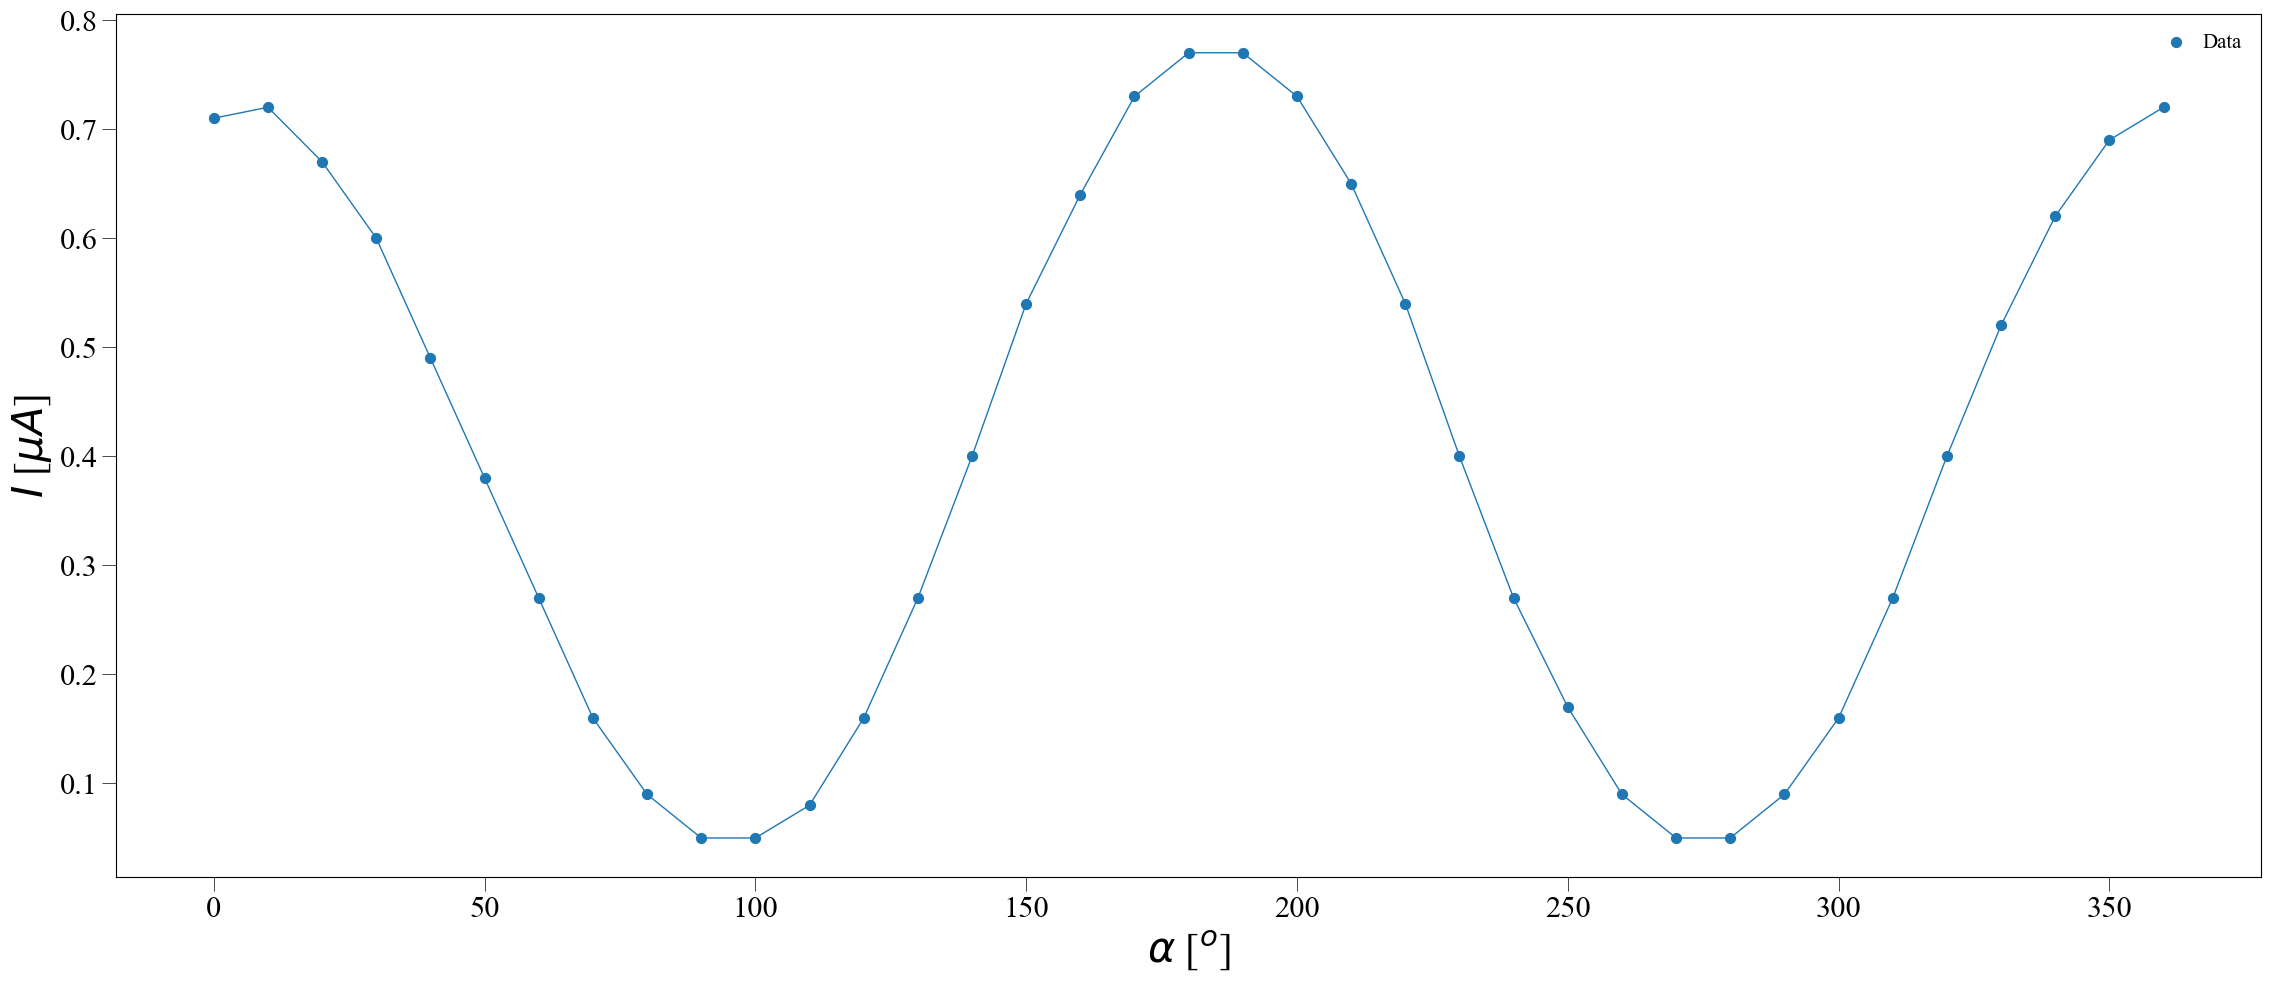
\includegraphics[scale=0.3]{intens}
                    \captionsetup{justification=centering, font=footnotesize}
                    \captionof{figure}{Závislost intenzity světla $I$ dopadajícího na detektor na úhlu natočení polarizátoru $\alpha$.}
                    \label{fig:intens}
                \end{figure}
    \begin{minipage}[t]{0.5\textwidth} 
                Z grafu byly získány následující hodnoty maximálních a minimálních intenzit $I_{max}$ a $I_{min}$:
                \begin{center}
                    $I_{max}$ = 0.77(1) $\mu$V
                    \vspace{5pt}
                    \par $I_{min}$ = 0.05(1) $\mu$V
                \end{center}
                Hodnota stupně polarizace se zjistí podle vzorce (6): 
                \begin{equation}
                    V = \frac{I_{max} - I_{min}}{I_{max} + I_{min}}
                \end{equation}
                Pak dostaneme:
                \begin{center}
                    $V$ = 0.88(2)
                \end{center}
                \par K výpočtu veličin a jejich nejistot byla použita knihovna Uncertinties pro Python: \href{pypi.org/project/uncertainties}. Kód je přiložen k protokolu. Chyby byly rozšířeny o Studentův koeficient (2-Tail Confidence Level) s ohledem na stupně volnosti pro každou hodnotu, pro interval spolehlivosti 99\%.
        \section{Závěr}  
            \subsection{Optická aktivita látek}
                Byly změřeny indexy lomu $n$ pro diionizovanou vodu a pro -0.1\% $n_{0\%} = 1.3324(1)$, 5\% $n_{5\%} = 1.339(2)$, 10\% $n_{10\%} = 1.346(1)$ a 15\% $n_{15\%} = 1.354(1)$. 
                \par Zmeřili jsme concentrační závislost indexu lomu $n$ a lineárně ji aproximovali, čímž jsme získali hodnotu $A$ = 0.0016(1). Dále jsme získali hodnotu úhlu lomu čisté vody $n_{voda}$ = 1.3324(1).
    \end{minipage}
    \hspace{10pt}
    \begin{minipage}[t]{0.5\textwidth} 
                Na základě této hodnoty úhlu lomu jsme vypočítali koncentrace $c_{vypoč.}$ vypočítané z naměřených hodnot indexu lomu $n$: -0.4(7)\%, 5(1)\%, 9.8(8)\% a 15.5(8)\%.
                \par Dále byla změřena specifická stáčivost $[\alpha]$ pro jednotlivé roztoky sacharózy: $[\alpha]_{5\%}$ = 75(7) $\frac{^o cm^3}{g ~dm}$, $[\alpha]_{10\%}$ = 80(5) $\frac{^o cm^3}{g ~dm}$ a $[\alpha]_{15\%}$ = 72(2) $\frac{^o cm^3}{g ~dm}$.
            \subsection{Malusův zákon}
                Byla změřena závislost intenzity světla $I$ dopadajícího na detektor na úhlu natočení polarizátoru $\alpha$. Z grafu byly získány následující hodnoty maximálních a minimálních intenzit $I_{max}$ a $I_{min}$: $I_{max}$ = 0.77(1) $\mu$V a $I_{min}$ = 0.05(1) $\mu$V. Hodnota stupně polarizace je $V$ = 0.88(2).
    \end{minipage}
\newpage
    \par K výpočtu chyb byl použit následující kód: 
    \begin{lstlisting}[language=Python, basicstyle=\tiny, breaklines=true, postbreak=\mbox{\textbackslashspace}]
        #Importing the libraries

        import matplotlib.pyplot as plt
        import numpy as np
        import pandas as pd
        from scipy import stats
        from scipy.stats import t as t 
        from scipy.optimize import curve_fit
        from uncertainties import *
        from uncertainties.umath import *
        
        #Reading data

        zero = pd.read_excel('data/0.xlsx')
        five = pd.read_excel('data/5.xlsx')
        ten = pd.read_excel('data/10.xlsx')
        fifteen = pd.read_excel('data/15.xlsx')
        alpha = pd.read_excel('data/alpha.xlsx')
        int = pd.read_excel('data/int.xlsx')

        out = pd.read_excel('data/out.xlsx')

        # Constants and values

        d = 0.01 #dm

        A_c = ufloat(0.0014, 0.00003)

        def uncert(data_input, uncert_inst):
            t_coeff = t.ppf((1 + 0.99)/2, len(data_input)-1)
            return np.sqrt((np.std(data_input)/np.sqrt(len(data_input)))**2 + uncert_inst**2)*t_coeff

        # Calculation 

        # Calculation 

        zero_c = ufloat(np.mean(zero['c']), uncert(zero['c'], 0.025))
        zero_n = ufloat(np.mean(zero['n']), uncert(zero['n'], 0.0001))
        five_c = ufloat(np.mean(five['c']), uncert(five['c'], 0.025))
        five_n = ufloat(np.mean(five['n']), uncert(five['n'], 0.0001))
        ten_c = ufloat(np.mean(ten['c']), uncert(ten['c'], 0.025))
        ten_n = ufloat(np.mean(ten['n']), uncert(ten['n'], 0.0001))
        fifteen_c = ufloat(np.mean(fifteen['c']), uncert(fifteen['c'], 0.025))
        fifteen_n = ufloat(np.mean(fifteen['n']), uncert(fifteen['n'], 0.0001))

        c_list = [zero_c, five_c, ten_c, fifteen_c]
        n_list = [zero_n, five_n, ten_n, fifteen_n]

        out['c'] = c_list 
        out['n'] = n_list

        alpha_0 = ufloat(np.mean(alpha['alpha_0']), uncert(alpha['alpha_0'], 0.01))
        alpha_5 = ufloat(np.mean(alpha['alpha_1']), uncert(alpha['alpha_1'], 0.01))
        alpha_10 = ufloat(np.mean(alpha['alpha_2']), uncert(alpha['alpha_2'], 0.01))
        alpha_15 = ufloat(np.mean(alpha['alpha_3']), uncert(alpha['alpha_3'], 0.01))

        alpha_list = [alpha_0, alpha_5, alpha_10, alpha_15]

        out['alpha'] = alpha_list
        out['alpha_corr'] = out['alpha'] - out['alpha'][0]

        out['c_corr'] = out['c'] - out['c'][0]
        out['c_corr'][0] = ufloat(-0.1, 0.025)
        out['alpha_corr'][0] = ufloat(-0.05, 0.01)
        
        out['alpha_prime'] = out['alpha_corr'] / (d*out['c_corr'])

        print(out) 

        I_max = ufloat(np.max(int['I']), 0.01)
        I_min = ufloat(np.min(int['I']), 0.01)

        V = (I_max - I_min) / (I_max + I_min)
        print('\nV = ', V)

        #Linear fitting

        # Calculate linear regression parameters
        slope, intercept, r_value, p_value, std_err = stats.linregress(out['c'].apply(lambda x: x.nominal_value), out['n'].apply(lambda x: x.nominal_value))
        A_fit_1 = ufloat(slope, std_err)
        n_0_fit = ufloat(intercept, std_err)
        print('A = ', A_fit_1)
        print('n_0 = ', n_0_fit)

        #Best fit line
        best_fit_line = slope * np.array(out['c'].apply(lambda x: x.nominal_value)) + intercept

        #Calculation of concentration

        out['c_calc'] = (out['n'] - n_0_fit) / A_c
        print(out)
    \end{lstlisting}
\end{document}